\documentclass[journal]{IEEEtran}

\usepackage[utf8]{inputenc}
\usepackage[T1]{fontenc}
\usepackage{amsmath,amssymb,amsfonts}
\usepackage{graphicx}
\usepackage{booktabs}
\usepackage{array}
\usepackage{url}
\usepackage[hidelinks]{hyperref}
\usepackage{orcidlink}
\graphicspath{{../figures/}}

\begin{document}

\title{One Image, Twelve Mathematics: A Cross-Family Benchmark and the U-Shaped
Editability of Image Representations}

\author{%
  Felipe Santib\'a\~nez-Leal~\orcidlink{0000-0002-0150-3246},~\IEEEmembership{Independent Researcher}%
  \thanks{F.\ Santib\'a\~nez-Leal is with the CAOS open-research programme, Santiago, Chile
    (e-mail: \texttt{fsantibanezleal@ug.uchile.cl}; ORCID: 0000-0002-0150-3246).}%
  \thanks{Preprint, 2026. Code, the committed derived artifacts, and the interactive lab are
    released under MIT at \url{https://github.com/fsantibanezleal/CAOS_IMGLAB}. Every external
    engine and reference carries its own license and citation; the explicit formulas shown are
    the author's own.}%
}

\markboth{Preprint, 2026 (v1.1) --- CAOS open-research programme}{Santib\'a\~nez-Leal:
One Image, Twelve Mathematics}

\IEEEtitleabstractindextext{%
\begin{abstract}
An image is always a matrix, but it can be re-expressed in many ways: as a sum over a Fourier,
cosine, or wavelet basis, as a sparse combination of atoms from an overcomplete dictionary, as a
handful of geometric primitives, as a small neural function of position, as an explicit closed-form
formula, or as a code in the latent space of a generative model. We carry one image across twelve
such families, on a common set of benchmark images and at a common parameter budget, and ask a
question the fidelity literature does not: when you edit the parameters, what happens to the image?
Two measured results and one finding follow. \emph{First}, at a comparable parameter budget the twelve
families reconstruct within a similar fidelity band (peak signal-to-noise ratio roughly $27$--$35$\,dB,
evaluated at each family's native resolution); fidelity does not sharply distinguish them. \emph{Second}, an editability-locality metric does: a single coefficient of a
global transform is spatially spread (Fourier $0.16$, DCT $0.23$ concentration) while a coefficient
of a space-localized transform is essentially local (wavelet $0.999$, KLT $1.0$). \emph{The finding}
is that editability is \emph{U-shaped} across the abstraction spectrum: it is high at two poles, the
designed-structure pole (geometric primitives, sparse atoms, space-localized transforms, where
humans built local meaningful coordinates) and the learned-manifold pole (disentangled generative
directions), and it collapses toward noise in between, where perturbing a raw neural-field weight or
a constant of a brittle fitted formula destroys the image. A parameter is both stable and meaningful
only when it indexes a low-dimensional manifold of plausible images with locally disentangled
coordinates. We give the twelve families with their governing equations, the cross-family benchmark
on six images, and the honest scope: arbitrary photographs do not reduce to compact, faithful,
human-readable equations, and the results say where a representation's parameters are, and are not, a
usable handle.
\end{abstract}

\begin{IEEEkeywords}
image representation, sparse coding, wavelets, KLT, implicit neural representation, Gaussian
splatting, symbolic regression, editability, rate-distortion, interpretability, reproducibility.
\end{IEEEkeywords}}

\maketitle
\IEEEdisplaynotcompsoctitleabstractindextext
\IEEEpeerreviewmaketitle

% =====================================================================
\section{Introduction}
% =====================================================================

\IEEEPARstart{A}{n} image is a matrix, but it is rarely stored or reasoned about as one. Compression
writes it in an orthonormal basis; a generative model writes it as a latent code; vector graphics
write it as shapes; parametric-equation art writes it as a formula. Each of these is a
\emph{representation}, a way to write an image as parameters, and each promises something different
about what those parameters mean. The forward question, how faithfully a representation reconstructs
the image at a given budget, is well studied. The question we ask is the inverse one: when you move
the parameters, does the image move in a stable, meaningful way, or does it fall apart?

We carry one image across twelve families of mathematical representation (Section~\ref{sec:families})
and measure two things on a common set of benchmark images at a common parameter budget
(Section~\ref{sec:bench}): fixed-budget fidelity, and an editability-locality metric. The result is
that fidelity is comparable across families and does not distinguish them, whereas editability does,
and it is organized as a U-shape across the abstraction spectrum (Section~\ref{sec:finding}). The
contributions are: (i) a single-image, twelve-family benchmark with each family's governing equation;
(ii) the measured editability-locality contrast between global and space-localized representations;
(iii) the U-shaped editability finding and its honest scope.

% =====================================================================
\section{The representation families}
\label{sec:families}
% =====================================================================

\textbf{Orthonormal transforms.} Fourier, DCT~\cite{ahmed1974} and wavelets~\cite{mallat1989} write
the image in a fixed orthonormal basis, $x=\sum_k c_k\phi_k$ with $c_k=\langle x,\phi_k\rangle$; the
map is exact and invertible, and keeping the top-$k$ coefficients gives the classical rate-distortion
tradeoff~\cite{wallace1992}. The KLT (PCA) replaces the fixed basis with the data-optimal basis
learned from image patches. A Fourier coefficient is a global grating; a DCT coefficient a per-block
frequency; a wavelet coefficient is local in space and scale.

\textbf{Overcomplete frames and sparse dictionaries.} Dropping orthonormality, a dictionary $D$ with
more atoms than pixels represents the image with a sparse code, $\min\lVert a\rVert_0$ s.t.\
$x\approx Da$, solved greedily by matching pursuit~\cite{mallat1993} on a learned or
overcomplete dictionary~\cite{aharon2006}. A related family uses \textbf{Gabor atoms}, oriented
Gaussian-windowed cosines~\cite{daugman1985}, each a legible object (position, width, orientation,
frequency, phase). Editing is local and semantic per atom, the first pole of high editability.

\textbf{Geometric primitives.} The image is approximated by an ordered list of translucent ellipses
fit greedily to the residual; each shape is an independent, meaningful, local coordinate.

\textbf{Implicit neural field.} A small coordinate network (SIREN~\cite{sitzmann2020}, with Fourier
features~\cite{tancik2020}) fits $f_\theta(x,y)\approx\text{image}(x,y)$; the image becomes the
weights $\theta$, continuous and resolution-free, but the parameters are entangled, no single weight
is a named handle.

\textbf{Symbolic closed-form.} Each channel is fit as an explicit trigonometric formula by ridge
regression on $D$ random Fourier features, $\text{ch}(x,y)=a_0+\sum_k[a_k\cos(\omega_k\!\cdot\!(x,y))
+b_k\sin(\omega_k\!\cdot\!(x,y))]$, linear in known analytic basis functions so the picture literally
is a readable equation~\cite{stanley2007}. Fidelity is honest and bounded: a smooth gradient reaches
$\approx57$\,dB from $512$ terms, a hard-edged checkerboard only $\approx14$, because a finite
trigonometric sum cannot render a discontinuity.

\textbf{Gaussian mixture (2D splatting).} The image is a sum of coloured anisotropic Gaussians,
$\text{ch}(x,y)=b+\sum_k c_k\exp(-\tfrac12 d_k^\top\Sigma_k^{-1}d_k)$, optimized jointly, the image
counterpart of the representation behind real-time radiance
fields~\cite{kerbl2023,gaussianimage2024}.

\textbf{Thin-plate radial basis.} A linear combination of a fixed thin-plate kernel plus an affine
plane, $\text{ch}(x,y)=a_0+a_1x+a_2y+\sum_i w_i\,\phi(\lVert(x,y)-c_i\rVert)$ with $\phi(r)=r^2\log r$,
the smoothest interpolant of scattered data~\cite{bookstein1989}, solved in closed form.

\textbf{Chebyshev series.} A truncated tensor polynomial series $\sum_{ij}a_{ij}T_j(x)T_i(y)$,
$T_k(t)=\cos(k\arccos t)$, fit live in the browser via discretely orthonormalized
moments~\cite{mukundan2001}; fidelity saturates on hard edges, the classical moments tradeoff.

\textbf{Fourier descriptors.} The dominant closed contour is traced and transformed into a sum of
rotating circles $z(t)=\sum_k c_k e^{if_k t}$, an exact orderable parametric description of a
one-dimensional curve.

\textbf{Generative latent.} The image is a code in the latent space of a variational
autoencoder~\cite{kingma2014}; the useful directions are disentangled and semantic, the second pole
of high editability.

% =====================================================================
\section{Cross-family benchmark}
\label{sec:bench}
% =====================================================================

\begin{figure*}[!t]
\centering
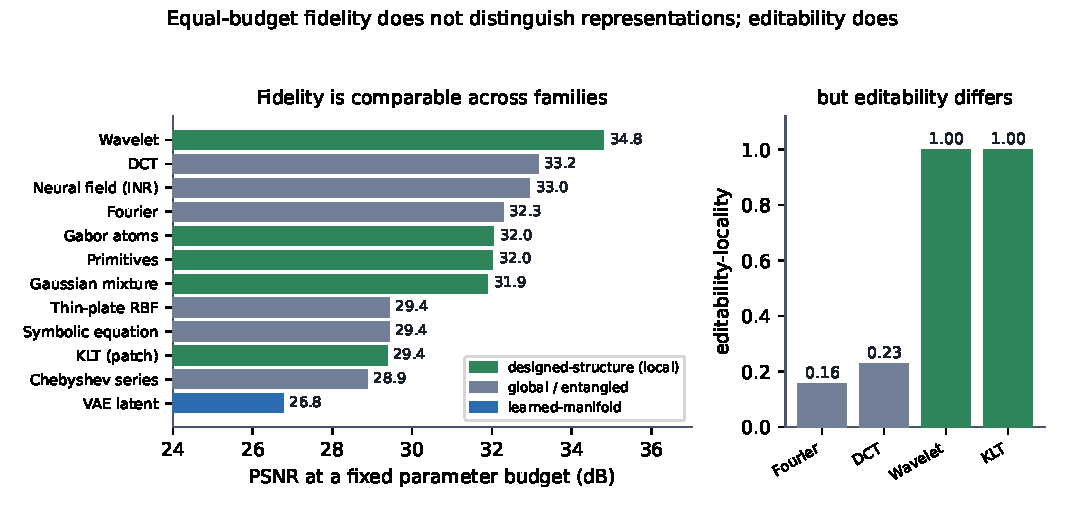
\includegraphics[width=0.98\textwidth]{fig-benchmark.pdf}
\caption{The benchmark, read from the committed \texttt{\_bench/index.json}. Left: peak
signal-to-noise ratio at a fixed parameter budget across the twelve families; fidelity is comparable
($27$--$35$\,dB) and does not distinguish them, coloured by pole (designed-structure local, global or
entangled, learned manifold). Right: the editability-locality metric for the four transform families;
a single coefficient of a global transform is spatially spread (Fourier $0.16$, DCT $0.23$) while a
coefficient of a space-localized transform is essentially local (wavelet $0.999$, KLT $1.0$).}
\label{fig:bench}
\end{figure*}

We bake each representation of six benchmark images (a photograph, a painting, a mathematical-art
image, an astronomical image, a texture, and a synthetic gradient) and evaluate two axes
(Fig.~\ref{fig:bench}); two further families described above, overcomplete sparse dictionaries and
Fourier-descriptor epicycles, appear in the interactive lab but are outside this fixed-budget
twelve-family benchmark. Each family is fit at its native working resolution (symbolic, Gabor,
Gaussian-mixture and thin-plate at $96$, the neural field and primitives at $128$, the four
transforms and the VAE at $256$), so the fixed-budget PSNRs below are not resolution-matched across
families and the fidelity comparison is qualitative rather than a strict ranking.
\emph{Fixed-budget fidelity}: at a comparable per-unit budget (matched by representational unit, not
scalar count: the top $5\%$ of transform coefficients, $\approx3300$ numbers, against $\approx1200$
ellipses, $\approx2300$ neural weights, $250$ Gabor atoms, $300$ Gaussians, $225$
thin-plate kernels, $512$ trigonometric terms, or a $4\times32\times32$ latent), the twelve families
land within $26.8$--$34.8$\,dB (wavelet $34.8$, DCT $33.2$, neural field $33.0$, Fourier $32.3$, Gabor
$32.1$, primitives $32.0$, Gaussian mixture $31.9$, thin-plate $29.4$, symbolic $29.4$, KLT $29.4$,
Chebyshev $28.9$, VAE latent $26.8$). Fidelity does not sharply separate the families. \emph{Rate-distortion}:
over coefficient fractions from about $2\%$ to $25\%$ the space-localized wavelet dominates (up to
$49.4$\,dB at $25\%$; DCT leads at the lowest $0.5$--$1\%$ fractions), then DCT and Fourier, with the
patch KLT lower, the classical energy-compaction ordering. \emph{Editability-locality}: we measure how spatially concentrated the effect of a single
coefficient is, operationally the fraction of a single coefficient's impulse-response energy that
falls within a fixed local neighbourhood ($1$ = perfectly local, $0$ = spread across the image; the
exact estimator and support size are in the released benchmark code); the global transforms are non-local (Fourier $0.156$, DCT $0.228$) while the
space-localized transforms are local-exact (wavelet $0.999$, KLT $1.0$). This is the axis on which the
families genuinely differ.

% =====================================================================
\section{The finding: U-shaped editability}
\label{sec:finding}
% =====================================================================

\begin{figure}[!t]
\centering
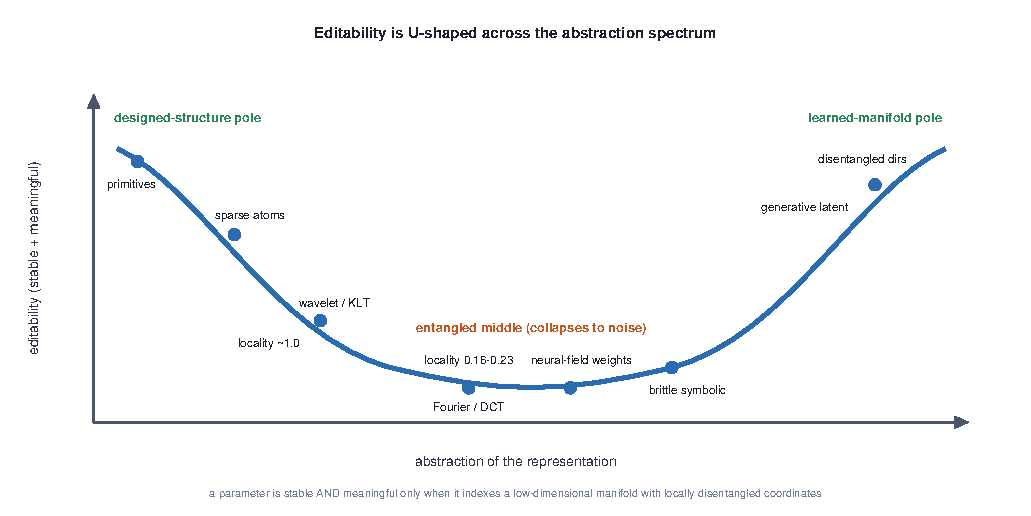
\includegraphics[width=\columnwidth]{fig-ushape.pdf}
\caption{Editability is U-shaped across the abstraction spectrum: high at the designed-structure pole
(primitives, sparse atoms, space-localized transforms) and the learned-manifold pole (disentangled
generative directions), and low in the entangled middle (global transforms, raw neural-field weights,
brittle fitted formulas).}
\label{fig:ushape}
\end{figure}

Putting the two axes together yields the finding (Fig.~\ref{fig:ushape}). Because fixed-budget
fidelity is comparable, what distinguishes the families for a user who wants to \emph{edit} the image
is whether a parameter is a stable, meaningful handle, and that is U-shaped across abstraction.
Editability is high at the designed-structure pole, geometric primitives (move one ellipse and only
that region changes), sparse and Gabor atoms (each a legible local object), and space-localized
transforms (wavelet and KLT, locality $\approx1$), because humans built local, meaningful
coordinates. It is high again at the learned-manifold pole, the disentangled directions of a
generative latent space, because the model learned a low-dimensional manifold of plausible images
with semantic axes. And it collapses in between: a single coefficient of a global transform is
spatially spread (locality $0.16$--$0.23$, so a local edit is impossible), a raw neural-field weight
is entangled (no weight is a named handle), and a constant of a brittle fitted formula is fragile
(perturbing it destroys the image, exactly because a finite trigonometric sum has no local support).
The organizing statement is that a parameter is both stable and meaningful only when it indexes a
low-dimensional manifold of plausible images with locally disentangled coordinates; the designed and
the learned poles achieve this by construction and by training, and the entangled middle does not.

% =====================================================================
\section{Discussion and honest scope}
% =====================================================================

The quantitative editability-locality is measured for the four transform families, where the
local-versus-global contrast is exact and unambiguous; the U-shape across all twelve families is the
organizing thesis, supported by that measurement, by the qualitative locality of each family's
parameters, and by the fixed-budget benchmark that rules out fidelity as the differentiator. The
result is descriptive, not a new representation: it says where a representation's parameters are, and
are not, a usable handle, which is the practical question behind interpretable and editable image
models. The honest scope is explicit: arbitrary photographs do not reduce to compact, faithful,
human-readable equations, the symbolic and formula families make genuine but bounded partial
reconstructions (a smooth gradient fits to $\approx57$\,dB, a hard edge to $\approx14$), and the
benchmark reports those partial results rather than overclaiming. The generative-latent pole is
argued from the disentanglement literature and the family's construction rather than from a locality
number, and is labelled as such.

% =====================================================================
\section{Conclusion}
% =====================================================================

We carried one image across twelve mathematical representation families on a common benchmark and
found that equal-budget fidelity does not distinguish them ($27$--$35$\,dB) while editability does,
and that editability is U-shaped across the abstraction spectrum, high at the designed-structure and
learned-manifold poles and low in the entangled middle, with the transform families' editability-locality
measured directly (global $0.16$--$0.23$ versus local-exact $\approx1$). A parameter is a usable
handle only when it indexes a low-dimensional manifold with locally disentangled coordinates. All
code and committed artifacts are released so the benchmark and the figures are reproducible.

% =====================================================================
\section*{Data and code availability}
% =====================================================================

Code, the committed benchmark artifacts, and the interactive lab are at
\url{https://github.com/fsantibanezleal/CAOS_IMGLAB} under the MIT license. Benchmark images are
public-domain or permissively licensed, plus procedurally generated license-clean images; each
carries its citation in the repository. Figure~\ref{fig:bench} is regenerated deterministically from the
committed \texttt{\_bench/index.json} by
\texttt{manuscripts/image-representation-editability/figures/make\_figs.py}; the U-shape schematic is
hand-authored (\texttt{fig-ushape.svg}).

\appendices
\section{Fixed-budget fidelity table}
At the matched budget the peak signal-to-noise ratios are: wavelet $34.8$, DCT $33.2$, neural field
(SIREN) $33.0$, Fourier $32.3$, Gabor atoms $32.1$, primitives $32.0$, Gaussian mixture $31.9$,
thin-plate RBF $29.4$, symbolic equation $29.4$, KLT (patch) $29.4$, Chebyshev series $28.9$, VAE
latent $26.8$\,dB, over six benchmark images (photograph, painting, mathematical art, astronomy,
texture, synthetic gradient). The full per-image rate-distortion curves and the editability-locality
values are committed in \texttt{data/derived/\_bench/index.json}.

% =====================================================================
\begin{thebibliography}{99}
\itemsep 1pt

\bibitem{ahmed1974} N.~Ahmed, T.~Natarajan, and K.~R. Rao, ``Discrete cosine transform,'' \emph{IEEE
Trans. Comput.}, vol.~C-23, no.~1, pp.~90--93, 1974, doi:10.1109/T-C.1974.223784.
\bibitem{mallat1989} S.~G. Mallat, ``A theory for multiresolution signal decomposition: The wavelet
representation,'' \emph{IEEE Trans. Pattern Anal. Mach. Intell.}, vol.~11, no.~7, pp.~674--693, 1989,
doi:10.1109/34.192463.
\bibitem{wallace1992} G.~K. Wallace, ``The JPEG still picture compression standard,'' \emph{IEEE
Trans. Consum. Electron.}, vol.~38, no.~1, pp.~xviii--xxxiv, 1992, doi:10.1109/30.125072.
\bibitem{mallat1993} S.~G. Mallat and Z.~Zhang, ``Matching pursuits with time-frequency
dictionaries,'' \emph{IEEE Trans. Signal Process.}, vol.~41, no.~12, pp.~3397--3415, 1993,
doi:10.1109/78.258082.
\bibitem{aharon2006} M.~Aharon, M.~Elad, and A.~Bruckstein, ``K-SVD: An algorithm for designing
overcomplete dictionaries for sparse representation,'' \emph{IEEE Trans. Signal Process.}, vol.~54,
no.~11, pp.~4311--4322, 2006, doi:10.1109/TSP.2006.881199.
\bibitem{daugman1985} J.~G. Daugman, ``Uncertainty relation for resolution in space, spatial
frequency, and orientation optimized by two-dimensional visual cortical filters,'' \emph{J. Opt.
Soc. Amer. A}, vol.~2, no.~7, pp.~1160--1169, 1985, doi:10.1364/JOSAA.2.001160.
\bibitem{sitzmann2020} V.~Sitzmann \emph{et al.}, ``Implicit neural representations with periodic
activation functions,'' in \emph{Adv. Neural Inf. Process. Syst. (NeurIPS)}, 2020, arXiv:2006.09661.
\bibitem{tancik2020} M.~Tancik \emph{et al.}, ``Fourier features let networks learn high frequency
functions in low dimensional domains,'' in \emph{Adv. Neural Inf. Process. Syst. (NeurIPS)}, 2020,
arXiv:2006.10739.
\bibitem{stanley2007} K.~O. Stanley, ``Compositional pattern producing networks: A novel abstraction
of development,'' \emph{Genet. Program. Evolvable Mach.}, vol.~8, pp.~131--162, 2007,
doi:10.1007/s10710-007-9028-8.
\bibitem{kerbl2023} B.~Kerbl, G.~Kopanas, T.~Leimk\"uhler, and G.~Drettakis, ``3D Gaussian splatting
for real-time radiance field rendering,'' \emph{ACM Trans. Graph.}, vol.~42, no.~4, 2023,
doi:10.1145/3592433.
\bibitem{gaussianimage2024} X.~Zhang \emph{et al.}, ``GaussianImage: 1000 FPS image representation
and compression by 2D Gaussian splatting,'' in \emph{Proc. Eur. Conf. Comput. Vis. (ECCV)}, 2024,
arXiv:2403.08551.
\bibitem{bookstein1989} F.~L. Bookstein, ``Principal warps: Thin-plate splines and the decomposition
of deformations,'' \emph{IEEE Trans. Pattern Anal. Mach. Intell.}, vol.~11, no.~6, pp.~567--585,
1989, doi:10.1109/34.24792.
\bibitem{mukundan2001} R.~Mukundan, S.~H. Ong, and P.~A. Lee, ``Image analysis by Tchebichef
moments,'' \emph{IEEE Trans. Image Process.}, vol.~10, no.~9, pp.~1357--1364, 2001,
doi:10.1109/83.941859.
\bibitem{kingma2014} D.~P. Kingma and M.~Welling, ``Auto-encoding variational Bayes,'' in \emph{Int.
Conf. Learn. Represent. (ICLR)}, 2014, arXiv:1312.6114.

\end{thebibliography}

\end{document}
